\documentclass{article}
\usepackage{amsmath, amsthm, amssymb, mathtools}
\usepackage{graphicx}
\newtheorem{theorem}{Theorem}

\title{Differential invariant signatures for planar Lie group transformations of
images}
\date{\today}
\author{Huey, Duey, and Louey}

\begin{document}
\maketitle



% TODO
%   SRM: Kiwi picture to Richard, paste text from disappear.tex
%   RGB: Images for mesh, and for signatures

\section{Introduction}
\subsection{Notation}
Let $G$ be a planar transformation group that acts on $k$-colour images $f
\colon \mathbb{R}^2 \rightarrow \mathbb{R}^k$ by $\varphi \cdot f \coloneqq
f \circ \varphi^{-1}$, where $\varphi \in G$.

When referring to coordinates, with $x \in \mathbb{R}^2$, we write $\hat{x}
= \varphi(x)$  and define the image post-transformation in the new
coordinates as
\begin{equation}
  \hat{f}(\hat{x}) = f(x).
\end{equation}
We derive relationships between the derivatives before and after
transformation by the chain rule:
\begin{equation*}
  f_{, i} = \hat{f}_{,k} \varphi_{k, i} 
\end{equation*}
etc. 





\section{The Stamp Collection I: The Affine group and its subgroups}
In this section we consider all the groups whose transformation is of the
form. For these groups, the change of variables formulae are, in tensor,
and matrix notations,
\begin{align}
  f_{,i} &= \hat{f}_{, k} a_{ki} & \nabla f &= A^T \nabla \hat{f} \\
  f_{,ij} &= \hat{f}_{, kl} a_{ki} a_{lj} & 
  \nabla^2 f &= A^T \nabla^2 \hat{f} A
\end{align}
$\varphi(x) = Ax + b$ for some matrix $A$ and vector $b$.

\subsection{SE(2)}
In this case we have $A^TA = I$ and $\det A = 1$.


\subsection{Invariants, hey!}
literature (Cartan, Olver, Russians, Draisma), motivation, etc,

\subsection{Invariants for images}
Colour and the lack of independence. Fractal dimension 

Calculating derivatives (discussion on desirability thereof).
Euclidean-invariant smoothing is a thing, other groups not so much.

\subsection{Introducing the cast}
Define each group, mesh image of what transformations can look like

\subsection{Technical wank}
Completeness, degeneracy, moving frames as concept table of numbers of
derivatives, all that jazz, maybe scaling technique
for dealing with invariants of non-unit weight


\section{The invariants}
One subsection for each group. Mathematical details/theorem/derivation, no
examples
\subsection{SA(2), E(2), SE(2), and Sim(2), or some better title}
\begin{theorem}
  SA(2) invariants up to second order are:
  I0, I1, I2 from Jupyter document
\end{theorem}

Corollary for E(2), SE(2), R2 and Sim(2)

Commentary on geometric interpretation of these things.
\subsection{A(2)}
\begin{theorem}
  General affine invariants using transvectants
\end{theorem}
Relative invariants and weights go here? probably

\subsection{M\"obius and Projective (finite dimensional)}
\begin{theorem}
  Moving frame invariants for M\"obius
\end{theorem}
\begin{theorem}
  Moving frame invariants for Projective
\end{theorem}

\subsection{Infinite dimensional diff groups (diff con, diff vol, diff)}




\section{Computational examples}
General idea of what we've done. Experiment to compare e.g. SA(2) and
Sim(2). Contrast between intuitive notion of complexity (described by
number of parameters in group) versus reality.

\subsection{Examples of all of 'em}
Big matrix of pictures for comparison purposes

\begin{figure}
	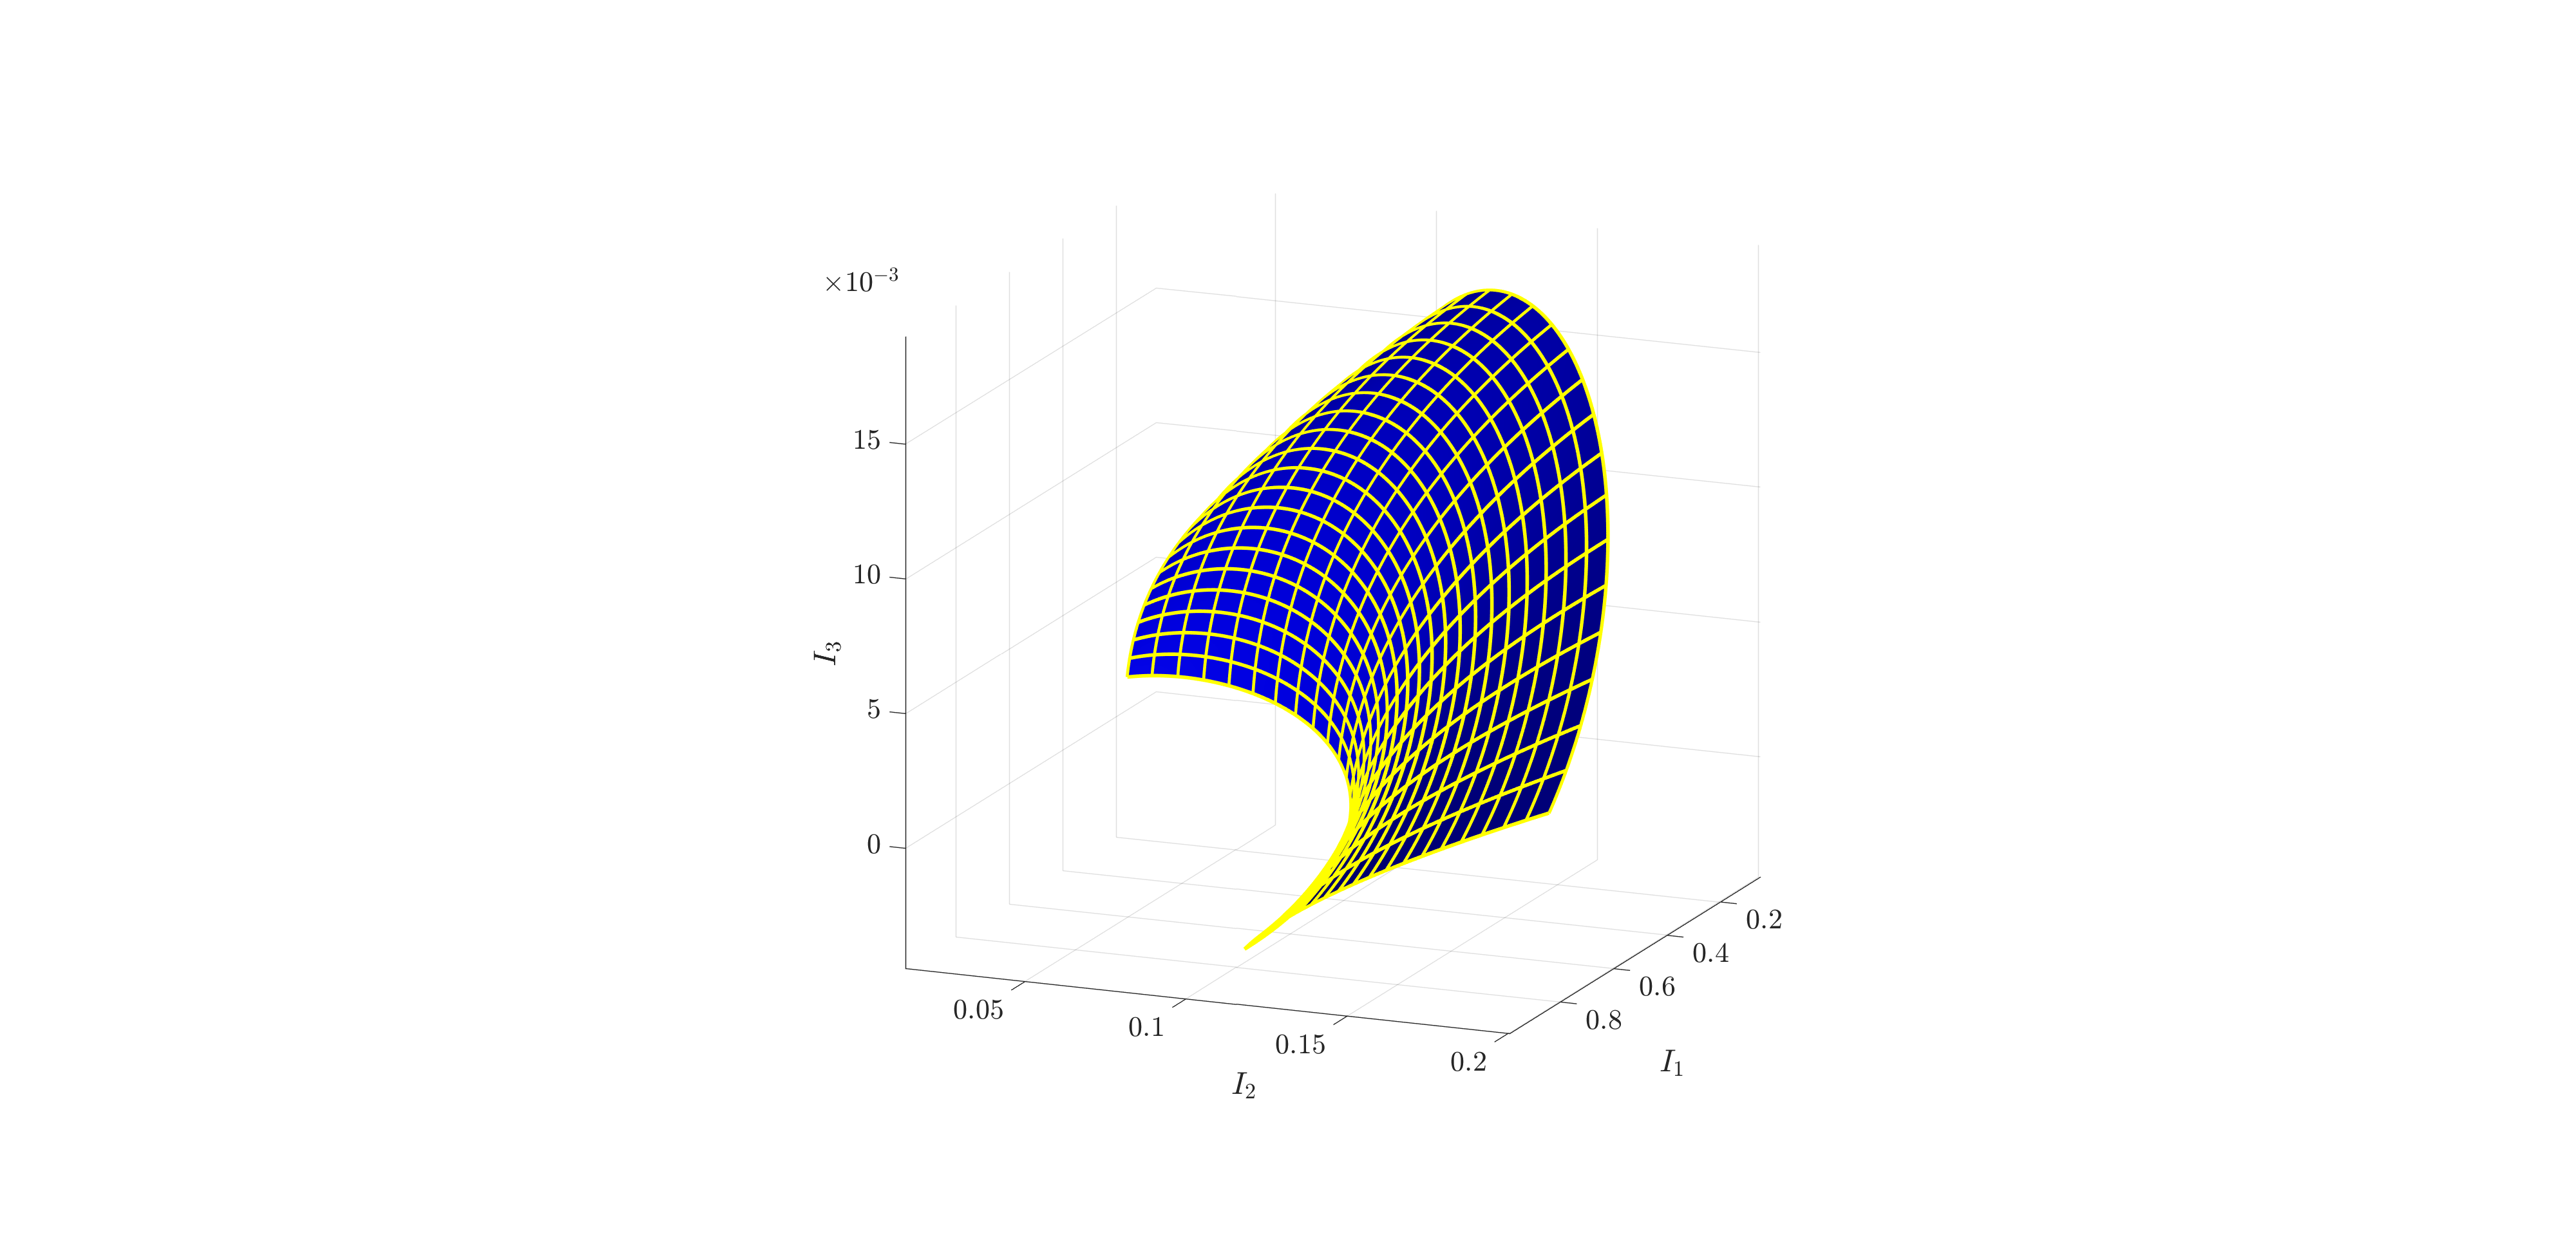
\includegraphics[width=12cm]{../images/SE2Transform_signature}
	\caption{SE(2) signature}
\end{figure}
\begin{figure}
	\includegraphics[width=12cm]{../images/E2Transform_signature}
	\caption{E(2) signature}
\end{figure}
\begin{figure}
	\includegraphics[width=12cm]{../images/SA2Transform_signature}
	\caption{SA(2) signature}
\end{figure}
\begin{figure}
	\includegraphics[width=12cm]{../images/A2Transform_signature}
	\caption{A(2) signature}
\end{figure}

\subsection{Hat tip to practicality: smoothing for E(2) and subgroups thereof}
Allows these groups to be used on real (i.e. not particularly
differentiable) images

\subsection{colour}

\section{Discussion and Conclusion or whatever}
Why are we using invariants? 
This idea is extremely local, can global information be better utilised?
Relation to using more computationally
tractable e.g. SA(2) not E(2)
Comparison with other invariant forms - e.g. Fourier, integral, etc.

\subsection{Future work}
Can we do better with the weights?
Can we do better with derivatives?
Projection onto Riemann sphere?
Noise. Ugh.

\end{document}
